\documentclass[journal]{IEEEtran}
\pagestyle{empty}
\usepackage{graphicx}

%
% Commands
%
\newcommand{\unit}[1]{\ensuremath{\, \mathrm{#1}}}

\begin{document}
\title{Studies of PLT-type Single-Crystal Diamond Pixel Detectors}

\author{
R.~Hall-Wilton~\IEEEmembership{CERN and ESS,}
M.~Gastal, R.~Loos, V.~Ryjov~\IEEEmembership{CERN,}
M.~Pernicka, H.~Steininger~\IEEEmembership{HEPHY~Vienna,}
K.~Andeen, A.~Barker, E.~Bartz, C.~Contreras-Campana, J.~Doroshenko, D.~Hidas, D.~Hits, R.~Patel, S.~Schnetzer, R.~Stone, P.~Thomassen~\IEEEmembership{Rutgers~University,}
V.~Halyo, B.~Harrop, A.~Hunt, D.~Marlow, D.~Stickland~\IEEEmembership{Princeton~University,}
W.~Bugg, M.~Hollingsworth$^*$\thanks{$^*$Speaker and contact: hollings@cern.ch}, T.~Robacker,  S.~Spanier, Z.~Yang~\IEEEmembership{University~of~Tennessee,}
A.~Delannoy, B.~Gabella, W.~Johns~\IEEEmembership{Vanderbilt~University,}
C.~Farrow~\IEEEmembership{University of Wisconsin}% <-this % stops a space
}

\maketitle
\thispagestyle{empty}

\begin{abstract}
The Pixel Luminosity Telescope (PLT) is a dedicated luminosity monitor, presently under construction and planned for installation during the next CMS opening, for the Compact Muon Solenoid (CMS) experiment at the Large Hadron Collider (LHC). It measures the particle flux in an array of sixteen telescopes each consisting of three layers of pixel diamond detectors. The PLT's single-crystal CVD diamonds are bump-bonded to the PSI46 pixel readout chip - the same readout chip used in the silicon pixel system in CMS.  Final hardware and software components have been assembled at CERN.  
The performance with has been measured this year in beams at the CERN PS, as well as the test beam facility at Fermilab.  With respect to charged particle tracking, we also measured the Lorentz angle in a magnetic field at the CERN SPS.  We present the results of these studies for the final system. 
\end{abstract}

%
% PLT
%
\section{Introduction}

The PLT is a dedicated luminosity monitor for CMS based
on single-crystal diamond pixel sensors which will be installed during the next CMS opening. It consists of two arrays of eight small-angle telescopes situated with one on 
each end of CMS.  The PLT is designed to provide a high-precision measurement of the bunch-by-bunch relative
luminosity at the CMS collision point on a time scale of a few seconds and a stable high-precision
measurement of the integrated relative luminosity over the entire lifetime of the CMS experiment.
 Figure~\ref{plt-location} shows a three dimensional design drawing 
of a PLT array. The telescopes consist of three equally-spaced planes of diamond pixel sensors with a total telescope 
length of 7.5~cm. They are located 5~cm radially from the beam line at a distance of 1.8~m from the central collision 
point with a small angle pointing towards the collision point.

\begin{figure}[!h]
\centering
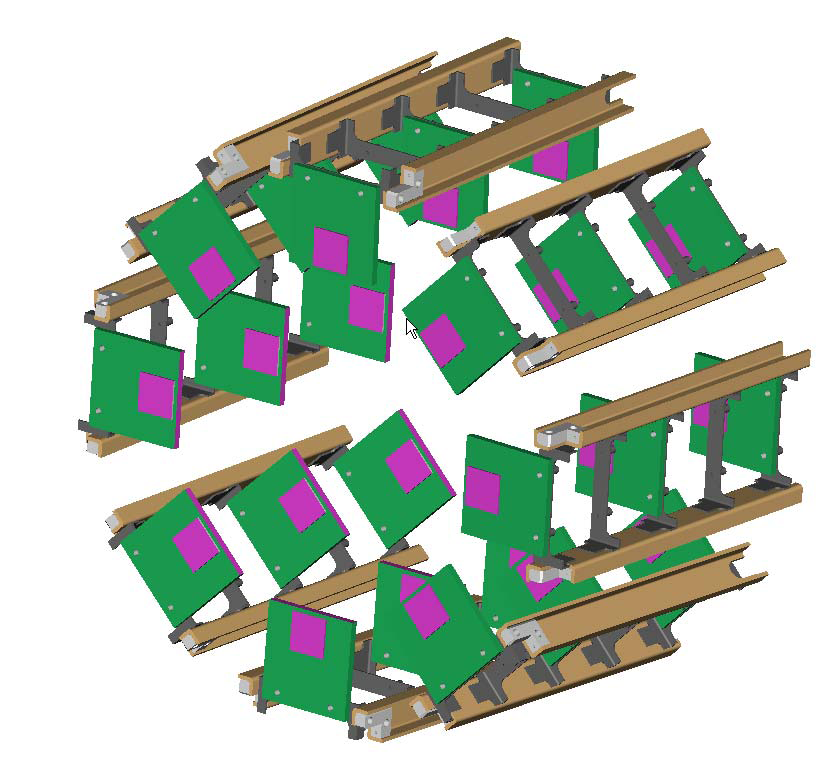
\includegraphics[width=0.45\textwidth]{PLT-Telescope}
\caption{3D design drawing of the telescope array at one side of the CMS detector, with the beam pipe in its center not shown. The length along the beam pipe between the outer two planes  is 7.5~cm. }
\label{plt-location}
\end{figure}

%
% sCVD
%
\section{Single-Crystal Diamond Detector}

Diamond sensors are crucial for the PLT application since they will operate efficiently with only
moderate decrease in signal size over the entire lifetime of CMS; they are capable of surviving up to $2\times10^{15}$ protons/cm$^2$~\cite{DiamondDetectors}. Of equal importance, this radiation hardness does not require that the sensors be cooled.  Furthermore, full charge collection typically occurs at an electric field of $<$ 0.2~V/$\mu$m across a 500 $\mu$m diamond.  
Single-crystal diamond is used for the sensor material rather than poly-crystal diamond due to its superior electrical properties; the larger height and narrower width of the collected charge distribution of single-crystal diamond ensures that any efficiency changes due to threshold
drifts will be small.

%
% Readout
%
\section{Detector Readout}
The telescope planes consist of single-crystal diamond sensors that are bump bonded to the PSI46.v2 CMS pixel readout
chip~\cite{psi46}.

The deposition of the pixel electrode pattern on the diamonds and the bump-bonding of the diamond
sensors to the pixel readout chips were performed at the Princeton Institute of Science and Technology 
Materials (PRISM) micro-fabrication laboratory. Following surface preparation, electrodes
were sputtered onto the diamond surface using a Ti/W alloy target as an under bump metalization. A 4 mm~$\times$~4 mm electrode was deposited on one side of the diamond using a shadow mask. 
On the other side, a pixel pattern was deposited using a standard lift-off photo-lithographic process. 
The pattern covered an area of 3.9 mm~$\times$~4.0 mm and consisted of an array of 26~$\times$~40 pixels 
with pitch of 150~$\mu$m $\times$~100 $\mu$m matching that of the PSI46 chip.

The PSI46 chip features individual pixel threshold/mask settings, full analog readout of the pixel hit address and charge deposit, as well as a column-multiplicity signal (known as the Fast-OR), which indicates the number of double columns that had pixels over threshold in each bunch crossing. 
The primary luminosity measurement of the PLT is based on counting the number of telescopes with three-fold coincidences formed from the Fast-OR output.  Fast-OR signals are read at the full bunch-crossing rate of the 40 MHz clock, while the full pixel
information, consisting of the row and column addresses and the pulse heights of all pixels over threshold,
is read out at a lower rate of a few kHz. This full pixel readout provides tracking information and
is a powerful tool for determining systematic corrections, calibrating pixel efficiencies and measuring
the real-time location of the collision point centroid.  The tracking capability and Fast-OR performance of the PLT  have been studied previously~\cite{pixel-2010}~\cite{ieee2010} and were found to be satisfactory for the application of the PLT.

The frontend for the full pixel readout is implemented in the same manner as the CMS pixel detectors are read out, which includes a Front End Driver (FED) and Front End Controller  (FEC)~\cite{control-readout}.  However, the Fast-OR information will be read out using customized FED firmware.  This firmware counts the number of threefold Fast-OR coincidences in each 25~ns bunch crossing window.  Each bunch crossing is referred to by its position relative to the start of the orbit. The result is a histogram of bunch number occupancies for each PLT telescope.   

The optical readout electronics consist of Hybrid Boards,  High Density Interconnects (HDI), Port Cards, and Optical Motherboards.  Hybrid boards are responsible for connecting directly to the PSI46 chip--one hybrid connects to one ROC.  Three hybrid boards connect to one HDI, and four HDIs connect to one Port Card.  The port card is then connected to the Optical Motherboard, which houses Analog Opto-Hybrids (AOH) and one Digital Opto-Hybrid (DOH).  AOHs turn the analog voltages into an optical signal which is forwarded to the FED, and DOHs are responsible for receiving commands from the FEC and relaying them to the other readout electronics.  Figure~\ref{fig:plt_cassette} shows half of the PLT detector for one side of the CMS detector as viewed from the center.

\begin{figure}[!h]
\centering
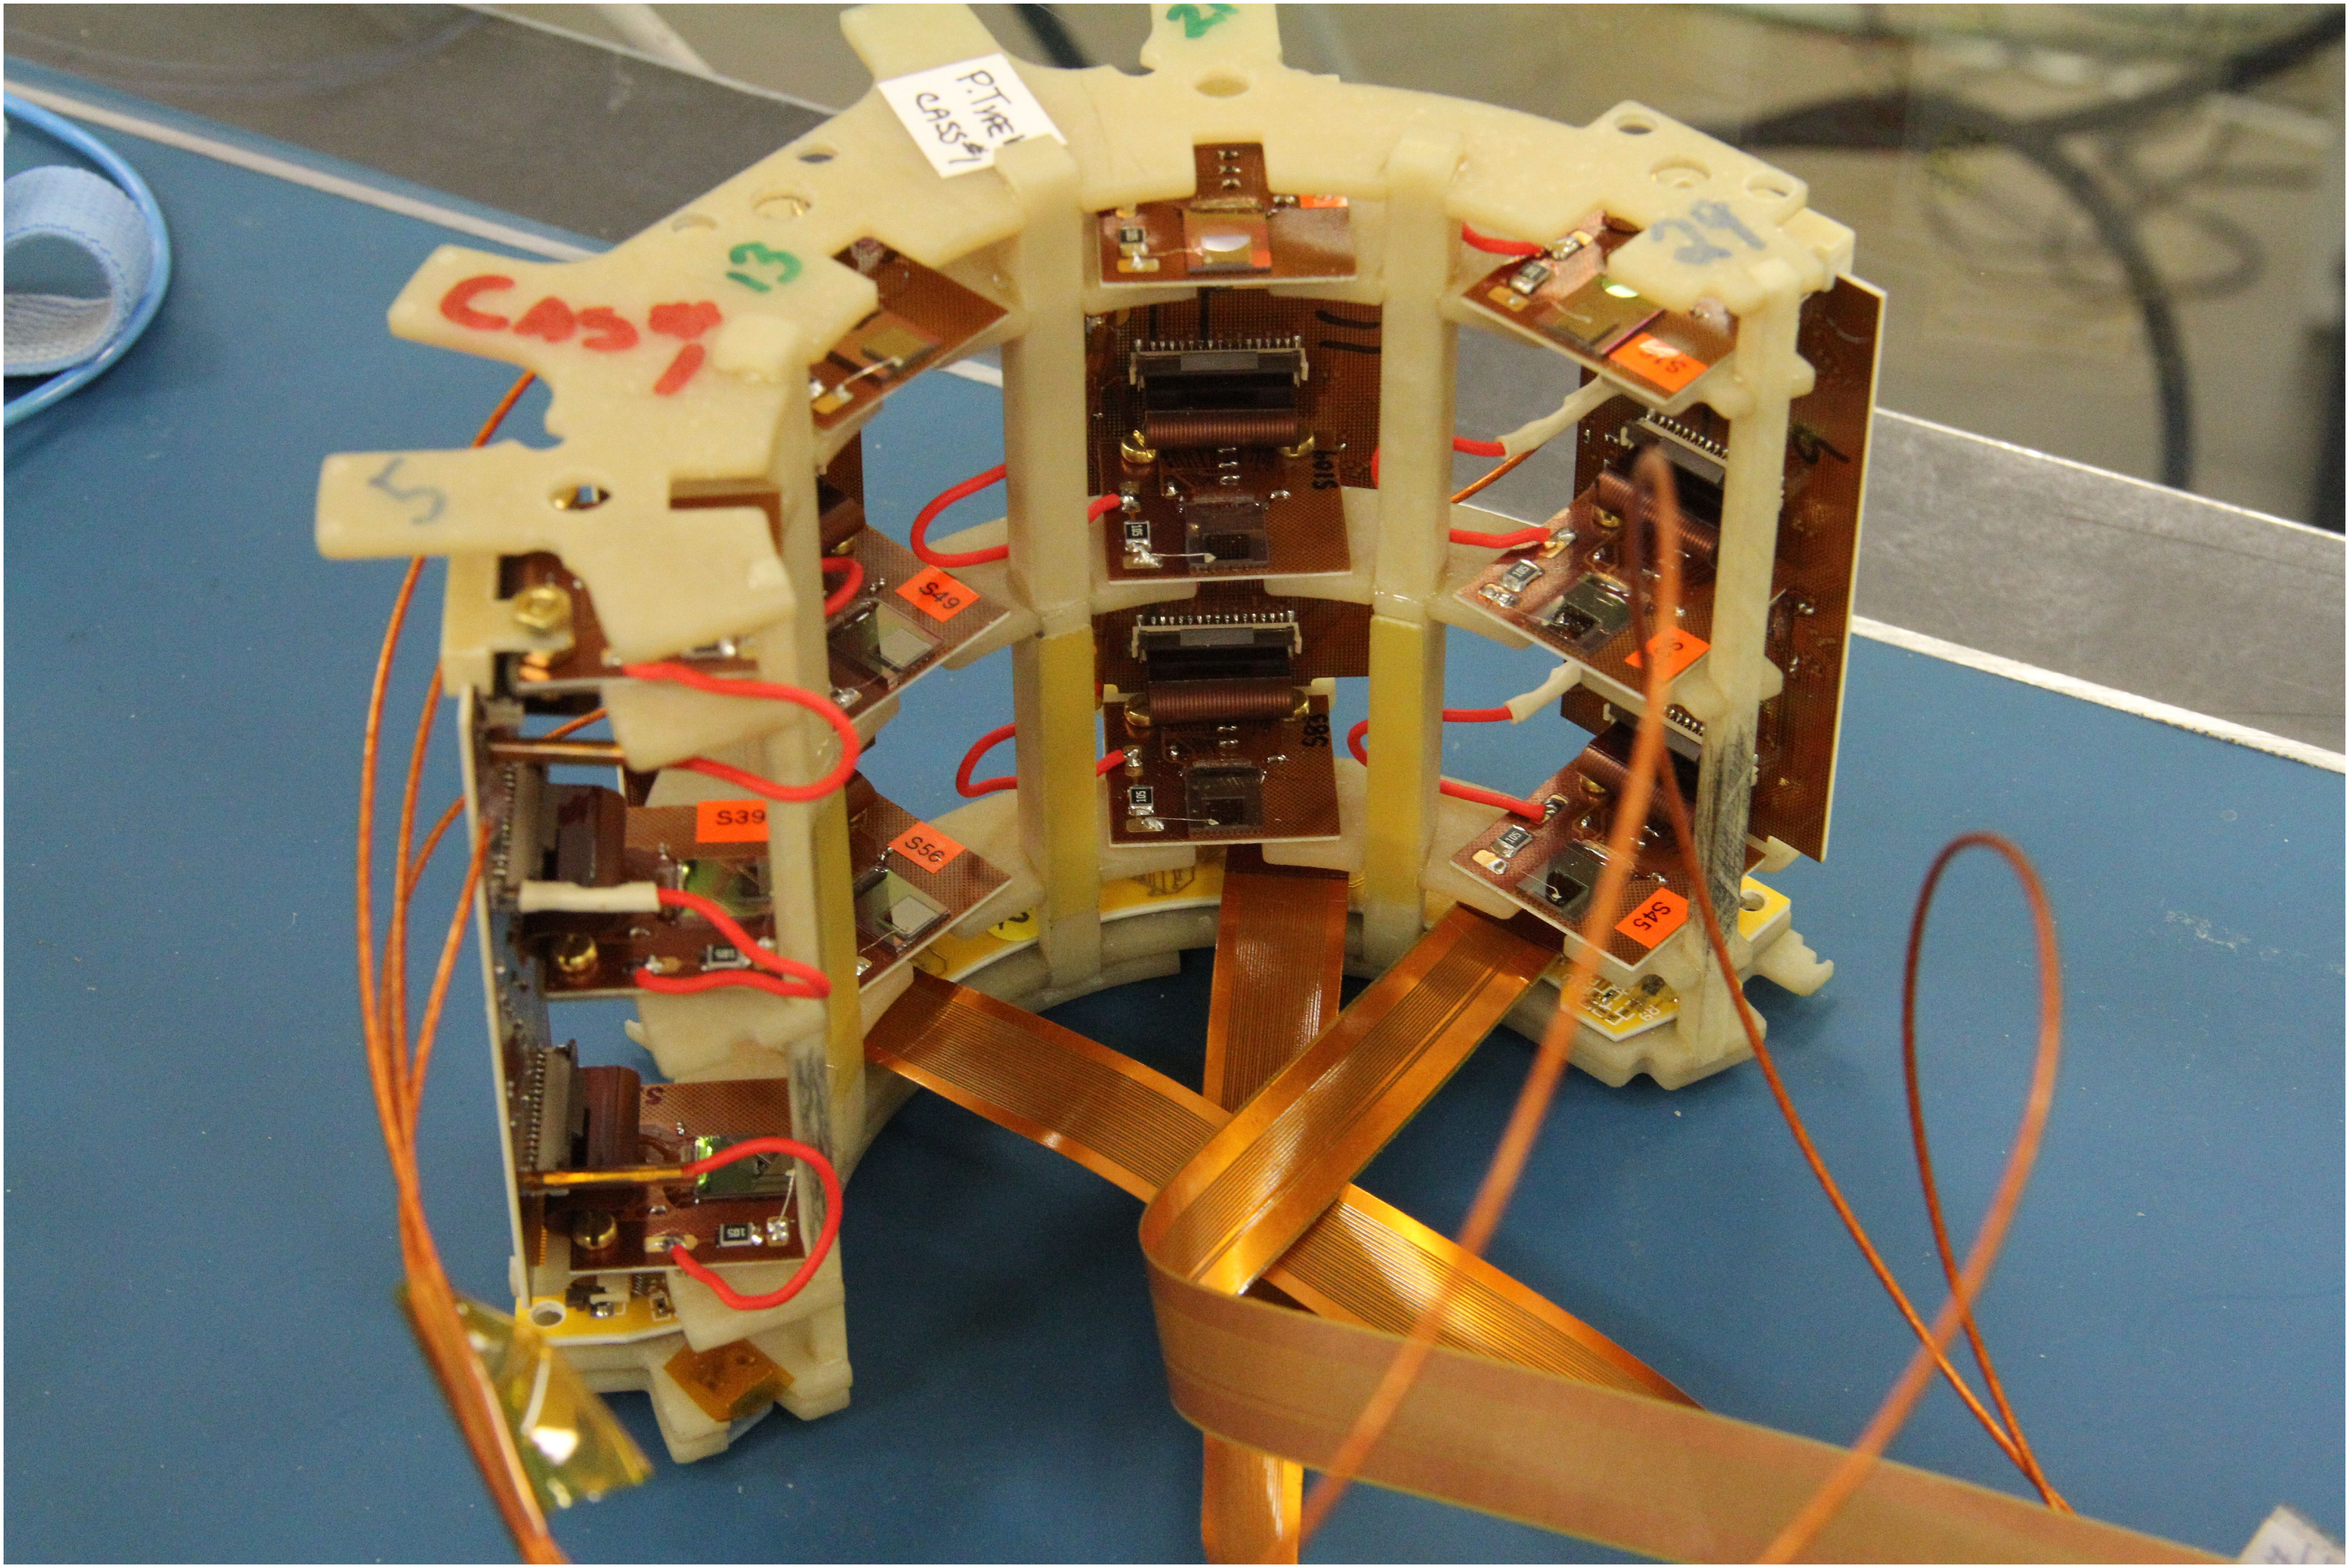
\includegraphics[width=0.45\textwidth]{plt_cassette}
\caption{ A fully assembled quarter of the PLT detector.  It consists of four three-plane telescopes.  }
\label{fig:plt_cassette}
\end{figure}


%
% Beam Tests
%
\section{Beam Tests}

 In order to test the final PLT components, we have carried out tests in the 10~GeV/c  beam of the CERN PS T9 beamline, in the 150~GeV/c beam of the CERN SPS H2 beamline, and in the Fermilab Test Beam Facility (FTBF).  The primary goals of these tests were to check the core functionality of the final PLT components, to characterize the performance of the customized FED firmware for luminosity measurement, and to test the system's robustness in a magnetic field. 
 
 The setup was also used to measure additional information to characterize the diamond pixel detector for particle tracking.  For this we performed a Lorentz angle measurement that requires the reconstruction of hit positions from the charge deposit pattern in the pixels inside a magnetic field of varying strength. These measurements utilized the Zurich Beam Telescope~\cite{zurich-telescope}.  For both the PS and the SPS tests, the PLT was set up in the middle of the four X/Y planes of the Zurich telescope such that two strip planes were upstream of the PLT and two were downstream.  At the FTBF, the Zurich telescope was not used, and the PLT was placed directly in the beam.
 
%\begin{figure}[!h]
%\centering
%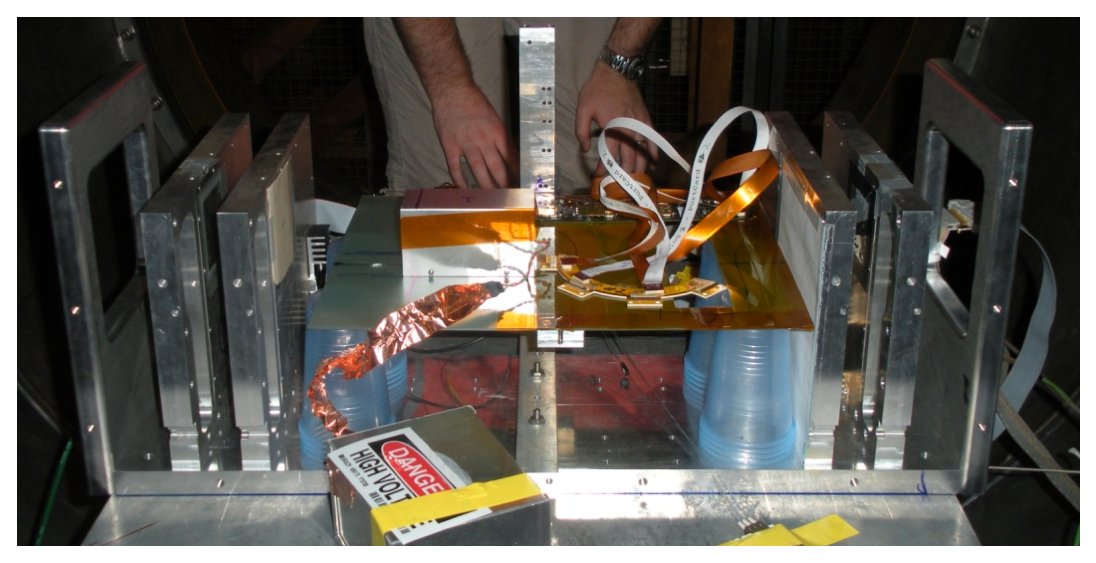
\includegraphics[width=0.45\textwidth]{sps-setup}
%\caption{ The PLT single-telescope assembly inserted into the Zurich Beam Telescope. }
%\label{fig:sps_setup}
%\end{figure}

%
% Fast OR firmware 
%
\section{Fast-OR Firmware Performance}
The Fast-OR FED Firmware was tested at the Fermilab Test Beam Facility.  The goal of this test was to measure the rate at which the firmware could reliably read out data and to test the histogramming functionality in the firmware.  The firmware was found to read out histogram data at a rate of up to 500 Hz.  This rate is sufficient for the PLT application, which requires a rate of $\approx 3$ Hz.   

The histogram functionality was tested by measuring the occupancy as a function of the bunch crossing number.  The bunch crossing number is defined as $(i \bmod N_{bunches}) - \Delta$, where $i$ is the clock cycle number, $N_{bunches}$ is the number of 25~ns cycles per orbit (3564), and $\delta$ is a phase parameter to ensure that bunch crossing zero occurs at the start of an orbit.  Since there is no correlation between the Fermilab beam clock and the PLT's 40~MHz clock, the per-bunch crossing occupancy was expected to be uniform in time.  Any non-uniformity would indicate a problem in firmware implementation.   Figure~\ref{fig:fastor} shows a single histogram for an arbitrary time window, demonstrating the expected uniformity.

\begin{figure}[!h]
\centering
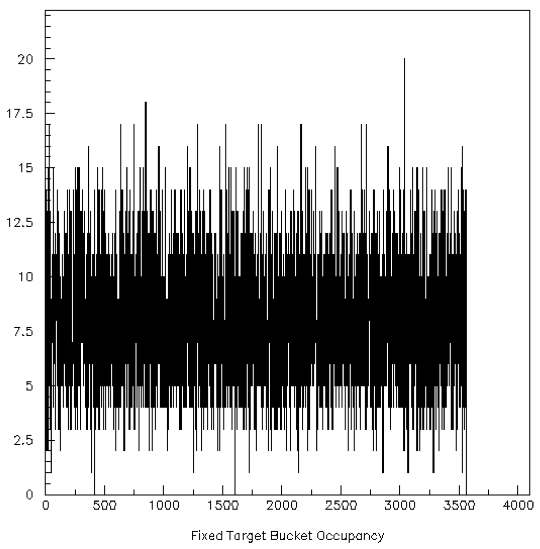
\includegraphics[width=0.45\textwidth]{histogram}
\caption{ The Fast-OR occupancy as a function of bunch crossing number over an arbitrary time window.  }
\label{fig:fastor}
\end{figure}

%
% Tracking
%
%\section{PLT Tracking performace}

 %
% Magnetic Field Stability
%
\section{Magnetic Field Stability}

To test the stability and performance of the PLT readout electronics when subjected to a magnetic field, a fully assembled cassette connected to a complete optical readout chain was inserted into a superconducting Helmholtz magnet at the CERN SPS H2 beam line.  This magnet is capable of reaching fields of $\pm 3$~Tesla.  Tests were run with different orientations of the PLT electronics inside of the field. 

In order to ensure that commands could be stably sent to the PLT at any field between 0T and 3T, a continuous gain calibration was run as the magnetic field ramped.  Ramping from 0 to 3 Tesla took approximately 3 hours, and ramping down took approximately 5 hours.  During that time, the calibration ran stably and no transmission errors were detected.  No degradation in the ADC signal was observed.

%
% Lorentz Angle
%
\section{Lorentz Angle and Electron Mobility}

An electrical charge that is moving in an 
electrical field perpendicular to a magnetic 
field is redirected with respect to the 
electric field direction. The angle between
the direction of electrical field and its
motion is the Lorentz angle.
The angle can be observed as a net smearing
of the position of the ionization charges generated
by a primary particle traversing the diamond detector
in a magnetic field (see Figure~\ref{fig:lorentz_measurement}).

\begin{figure}[!h]
\centering
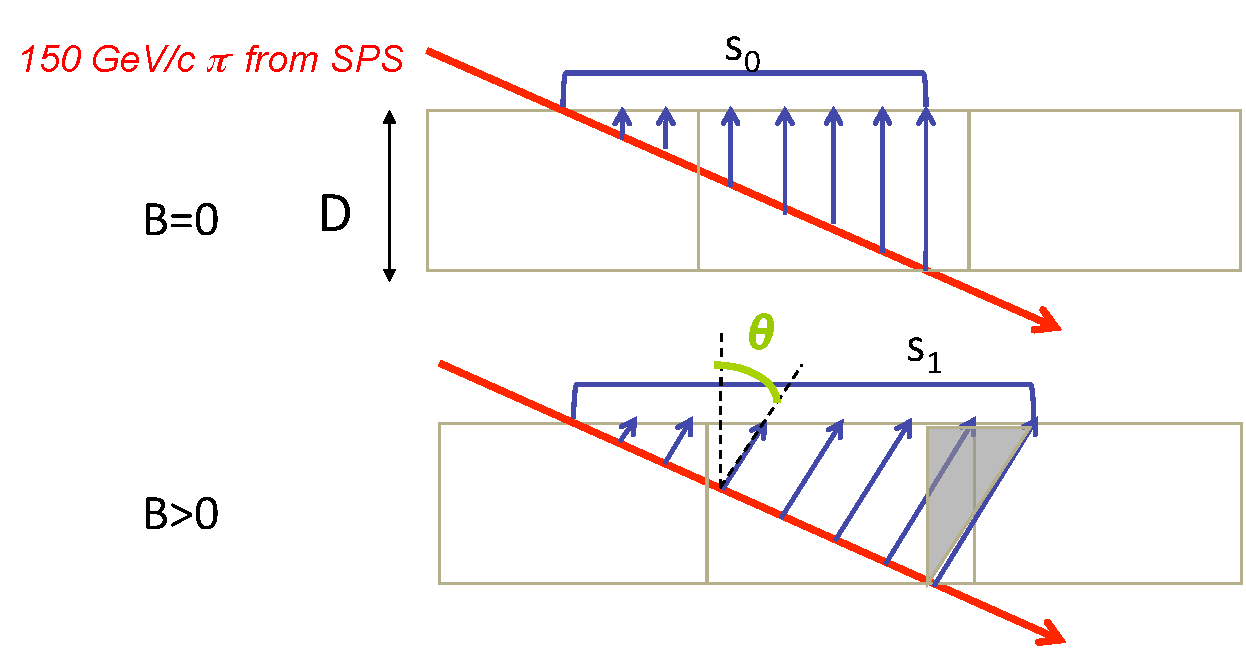
\includegraphics[width=0.48\textwidth]{lorentz_measurement}
\caption{ The strategy for measuring the Lorentz angle (drawing is not to scale).  The spread of the charge distribution, $s$, is measured by requiring two hits in the pixel detector and taking the difference between the charge-weighted position in the pixel detector and the track measured by the Zurich Beam Telescope.  The detectors were tilted 20~degrees with respect to the beam direction. }
\label{fig:lorentz_measurement}
\end{figure}

After the stability of the PLT in a magnetic field was confirmed, the PLT cassette was removed and replaced with a single three layer telescope configuration.  This setup included the Zurich Beam Telescope for precision tracking. For this test, the PLT planes were tilted by 20 degrees with respect to the beam direction such that charge sharing was enforced geometrically along the 100 $\mu$m pitch direction (the 100 $\mu$m direction is referred to as the Y direction and the 150 $\mu$m pitch is referred to as the X direction).  The magnetic field was oriented such that the field lines pointed along the X direction--the same configuration as the barrel pixel detector in CMS.
Both the Zurich Beam Telescope and the PLT were triggered by the center ROC's Fast-OR signal. During all tests, the diamonds were supplied a bias of 500 V, resulting in an electric field of 1 V/$\mu$m.  At this electric field, full charge collection is expected from all diamonds.
The goal of this setup was to measure the repositioning of the ionization charges in the pixel detectors.   In doing so, we also test the tracking capability of
the diamond pixel and the longer-term operational stability of
the readout chain.

%
% Zurich Beam Telescope Characterization
%
 \subsection{Zurich Beam Telescope Characterization}

The Zurich Beam Telescope is a silicon microstrip telescope, which consists of 4 planes of X/Y strip detectors.  The intrinsic resolution per-plane was measured at a previous test beam by C.~Amsler~\emph{et al.}~\cite{zurich-telescope} to be $\approx 2 \mu m$.   Strip readout is done through a multiplexed readout chain, where each strip reports its charge deposit as a pulse which is synced with a global clock and read out through an ADC.  The frontend electronics consist of an array of 5 VA2 128 channel preamplifiers per detector, which includes charge sensitive amplifiers and semi-gaussian shapers~\cite{zurich-telescope}.

Tracks through the Zurich Beam Telescope are defined completely independently in X and Y, except for the common requirement that there is exactly one set of adjacent strips in X and in Y.  Alignment is thus done on X and Y independently.  During alignment, all tracks consist of only 2-strip hits since they provide the most accurate position.  During all stages of reconstruction,  noisy strips are detected and removed by measuring occupancy in each strip; any strips which satisfy the requirement $o_i >  \bar{o}_{sideband} + 3\cdot RMS(o_{sideband})$ are tagged as noisy.  Here, $o_i$ is the occupancy of the $i$th strip, $\bar{o}_{sideband}$ is the mean of the occupancy of the 5 nearest neighbors on the left and right of the $i$th strip, and $RMS(o_{sideband})$ is the RMS spread of the same sideband distribution as used to find $o_{sideband}$.

A given plane was aligned with respect to a predicted track position based on the measurements in the remaining three layers.  The residual was calculated for each plane, where the residual is defined as $\Delta x = x_{track} - (x_{measured} - x_{offset})$.  Here $x_{track}$ is given by a projection of a  linear fit through the other 3 telescope planes, $x_{measured}$ is the measured position in the plate for which the residual is calculated, and $x_{offset}$ is the alignment offset.  The quantity $\chi^2 = \sum_{i=1}^4 \Delta x_i^2$ is then minimized as a function of $x_{offset}$ in order to find the alignment offsets.  At the PS, the data used for the final alignment was taken without the PLT assembly in order to minimize the multiple scattering contribution.  At the SPS, the multiple scattering contribution was negligible, so the full assembly was inserted. Data for alignment at the SPS was taken without magnetic field.

At the SPS, the residual after alignment was $<\Delta x> \approx$5 $\mu$m, resulting in a precision in the prediction of the hit position at the diamond detector of $\approx$ 2.5 $\mu$m.  Example residual distributions from the SPS run with and without magnetic field are shown in Figure~\ref{fig:bt_residuals}.

\begin{figure}[!h]
\centering
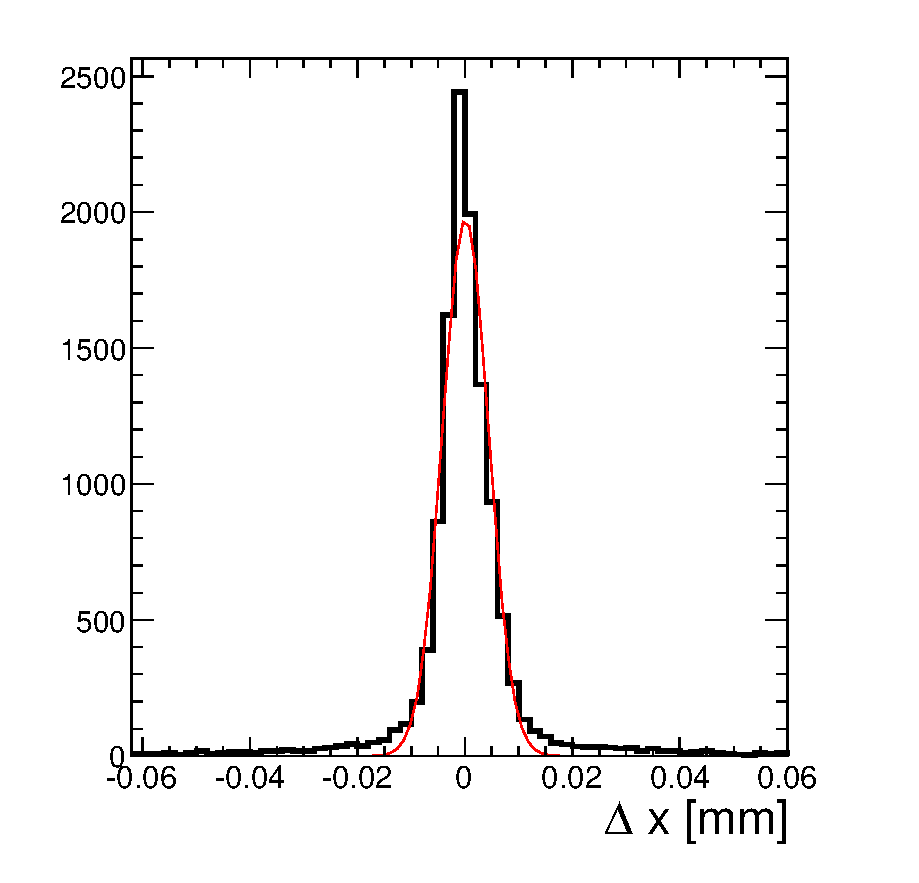
\includegraphics[width=0.45\textwidth]{bty-example}
\caption{ A typical residual distribution for a single Zurich Beam Telescope plane in no magnetic field. }
\label{fig:bt_residuals}
\end{figure}

\subsection{Lorentz Angle Measurement}

%The Lorentz angle may then be measured by finding the difference between the spatial spread at a given magnetic field and the spread with no magnetic field, as demonstrated in Figure~\ref{fig:lorentz_measurement}.  
%A single track crossing is defined by a clustering algorithm in which all contiguous above-threshold pixels are considered part of a single track crossing.  This series of above-threshold pixels is called a cluster.  

The position of the track in the diamond detector was
measured with the Zurich telescope. 
A single track crossing in the PLT is defined
as a continuous series of pixels with charge deposits above 
threshold--also called cluster. The charge-weighted position provided by the cluster is then calculated by the formula 

\begin{equation}
Y = \frac{\sum_i y_i \cdot Q_i}{\sum_i Q_i}
\end{equation}

An analogous equation is used for X.  Here, $Q_i$ is the charge in the ith pixel and $y_i$ is that pixel's position.

Due to the redirection of the ionization charges in the magnetic
field the observed signal at the readout side of the diamond detector
is smeared along the Y direction. 
The Lorentz angle can be measured from the difference between the extent of the charge deposit along the detector, referred to as the
spatial spread $s(B)$, at a given magnetic field and the spread with no
magnetic field $s_0$ (see Figure~\ref{fig:lorentz_measurement}),

\begin{equation}
\tan\theta_L = 	\frac{\bar{s}(B) - \bar{s}_0}{D} = \frac{\bar{v}_d \cdot B}{E} = \bar{\mu}\cdot B
\end{equation}

where $\theta_L$ is the Lorentz angle,  $D$ is the thickness of the diamond (500 $\mu$m for the PLT sensors), $\bar{s}(B)$ is the average value of the size of the spread of the charge distribution as a function of the magnetic field, $s_0$ is the spread with no magnetic field, $v_d$ is the drift velocity, $B$ is the magnetic field, $E$ is the electric field, and $\bar{\mu}$ is the average mobility.

The spatial spread of the charge distribution $s(B)$ is twice
the residual between the PLT charge centroid and the track 
entrance position predicted by the Zurich telescope, $\Delta Y$:

\begin{equation}
s(B) = 2 \cdot \Delta Y
\end{equation}

For measuring the Lorentz angle, it was required that there is $>1$ hit in the cluster, that there is no extension of the cluster in the X direction, that all pixels in the cluster were more than two pixels away from the border, and that all four Zurich Beam Telescope planes registered exactly one hit in $X$ and $Y$.  We require also that the pixel hit position in $X$, as predicted by the strip telescope, stays more than $30 \mu$m away from the pixel border. 
%We measure $\bar{s}(B)$ by taking the difference between the track entrance position as given by the Zurich Beam Telescope and the charge-weighted cluster position in the diamond detector.

% Spread: The extent of the charge along the pixel, or spread

The measured values of $\bar{s}(B)$ are shown in Figure~\ref{fig:offsets}.    The point at $-1$ T was not included due to lack of statistics, and at $-3$~T because it was found that the Lorentz angle was partially compensated by the geometrical tilt, resulting in primarily one hit clusters.   

The uncertainty on the magnetic field corresponds to an uncertainty of $\pm 10$A of the magnet current; the field of 3T corresponds to a current of $4000$A.  The uncertainty on the 1T measurement is larger since, due to time constraints, data were taken while the magnet was still ramping down.


The extent by which a cluster spreads depends on the amount of 
deposited charge and the threshold setting in a given pixel. 
As the position of the primary particle moves along the direction 
of the smearing $Y$ the position reconstructed from the PLT cluster 
falls behind. This is due to the delayed onset of the pixel in this 
direction until its charge deposit exceeds the threshold in that pixel.
The higher the threshold setting the larger this retardation.
On the opposite side of the cluster the pixel drops out faster
the higher the threshold setting. Then the cluster-based position
moves ahead of the position predicted by the strip telescope.
Both effects average out over a large sample if the illumination of 
the detector is uniform and the thresholds are not systematically 
mis-set across the detector.  Figure \ref{fig:occupancy} shows the occupancy along the axis of the Lorentz smearing, which depends on the the combination of illumination and thresholds.  No substantial inefficiency was observed. 

\begin{figure}[!h]
\centering
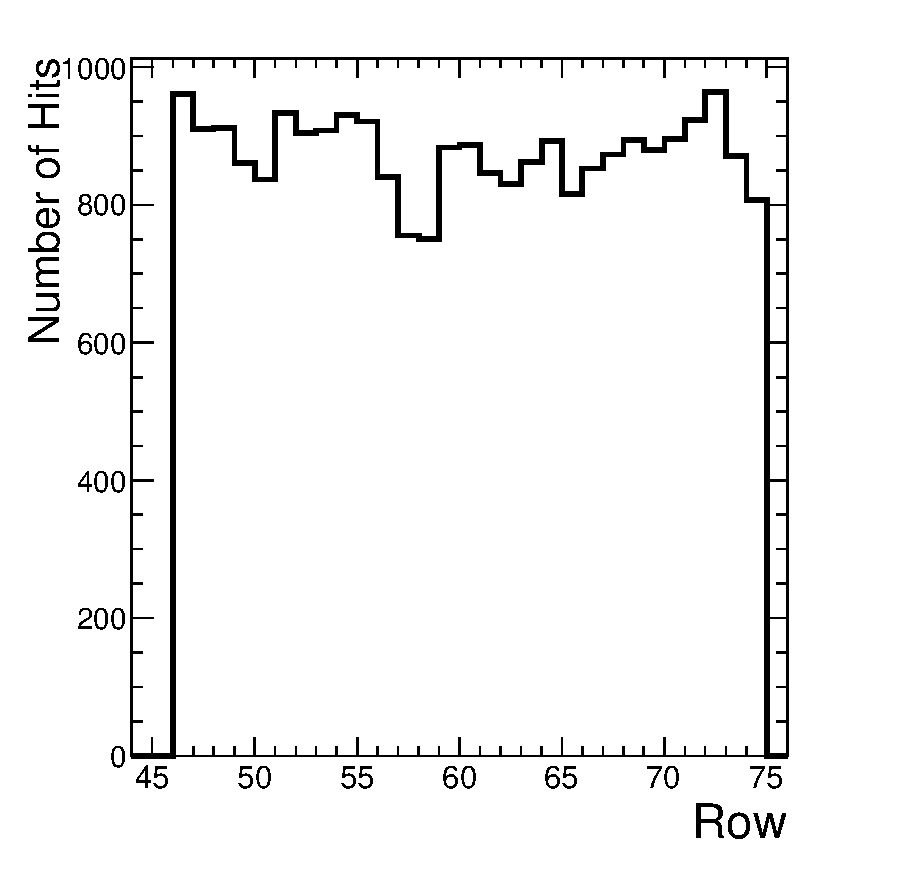
\includegraphics[width=0.5\textwidth]{plt_row_occupancy}
\caption{ The number of reconstructed hits per pixel projected along the direction of the Lorentz smearing.}
\label{fig:occupancy}
\end{figure}
 
The uncertainty on the $\bar{s}(B)$ values has several contributions:
We consider an uncertainty in the centroid due to asymmetries in the $s(B)$ distribution.  We calculate the difference between the positions where the integrated normalized s-distribution is at the 10\% ($s_1$) and 90\% ($s_2$) level with respect to the mean ($\bar{s}$): $\Delta = s_1 + s_2 - 2\bar{s}$. We adopt the full shift $\Delta$ as error. We estimate the uncertainty due to the integration over the $X$ direction from the variation of the centroid when removing the requirement on $X$ position. The total error shown in Figure~\ref{fig:offsets} is the quadratic sum of the last two contributions and the statistical error on the centroid.    We performed detector alignment with zero magnetic field
data taken before and after the magnet ramp.
Contributions from tracking in the strip telescope and 
alignment were found to be negligible. 
We fit those measurements to a first order polynomial. The result is shown together with the data points in
figure~\ref{fig:offsets}.

%\begin{table}[htdp]
%\caption{Sources of Uncertainty}
%\begin{center}
%\begin{tabular}{|c|c|c|c|}
%B [T] & Asymmetry [$\mu$m] & $\sigma_{mean}$ & X restriction \\
%-2 & 6.1 & 3.1 & 7.0 \\
%0 & -2.0 & 0.1 & 2.2 \\
%1 & 0.4 &-3.3 & -1.0 \\
%2 & 8.8 & 2.5 & 5.6 \\
%3 & 16.0 & 3.0 & 0.1 \\
%\end{tabular}
%\end{center}
%\label{default}
%\end{table}%


The mobility of free charge carriers in our sensor is given by the
slope, $\frac{\Delta s}{\Delta B}$, the following:

\begin{equation}
\frac{\Delta s}{\Delta B} \equiv \alpha = \bar{\mu} \cdot D \rightarrow \bar{\mu} = \frac{\alpha}{D}
\end{equation}

Assuming that our measurement is dominated by the collection of electrons on the side of the ROC, we yield an average mobility for those charge carriers of  $596 \pm 101 $ cm$^2$/Vs, corresponding to a drift velocity of $5.96 \times 10^4$~m/s.  This measurement can be compared to previous measurements using different techniques such as the transient current method~\cite{diamond-mobility}, who found an electron mobility of $\approx$ $650$ cm$^2$/Vs.  We expect therefore a Lorentz angle of $\theta_L = (13.4 \pm 2.1)^\circ$  in a magnetic field of 4T and an applied bias of $1$V/$\mu$m for a barrel-type diamond pixel detector.



\begin{figure}[!h]
\centering
%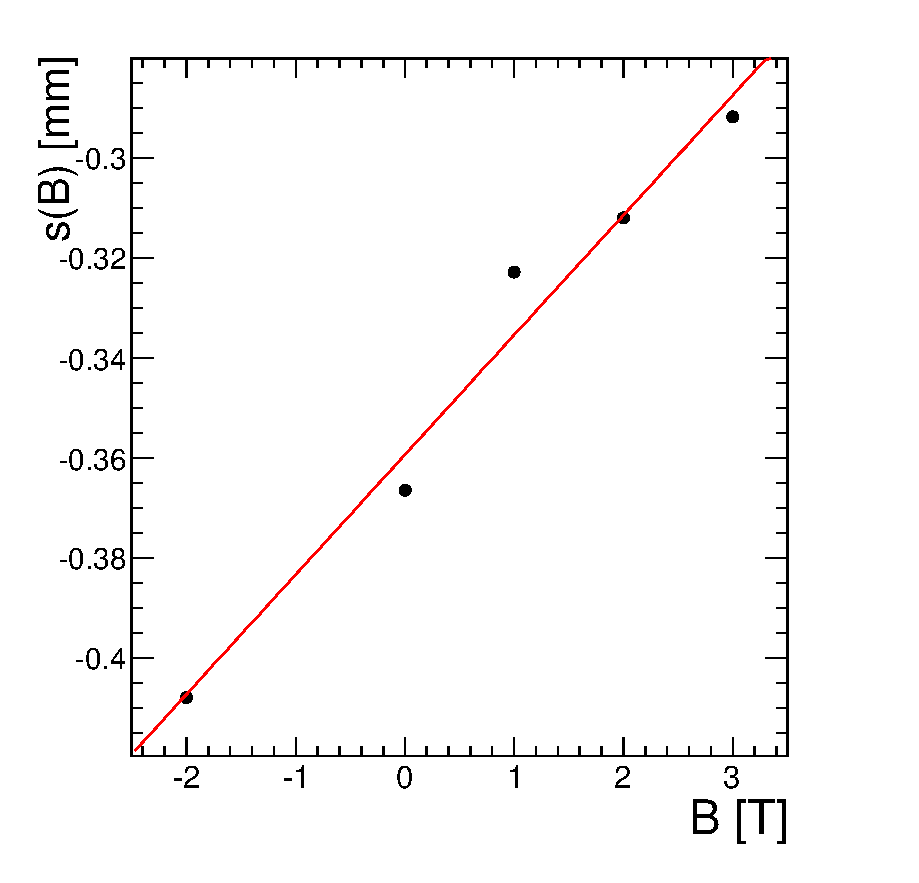
\includegraphics[width=0.5\textwidth]{plt-lorentz-offsets-v4}
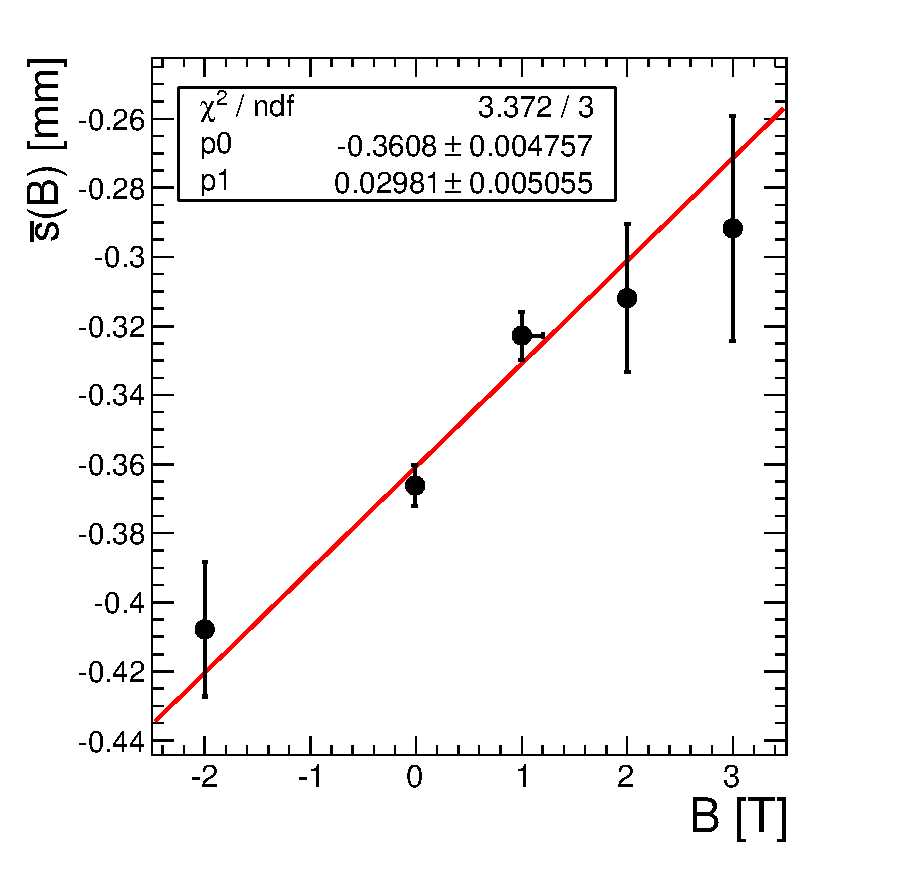
\includegraphics[width=0.5\textwidth]{plt-offsets-with-errors}
\caption{ The spatial spread along the direction of the Lorentz drift as a function of B.  The red line is a first-degree polynomial fit of the data, the slope of which is proportional to the electron mobility in single-crystal diamond. }
\label{fig:offsets}
\end{figure}



%\begin{figure}[!h]
%\centering
%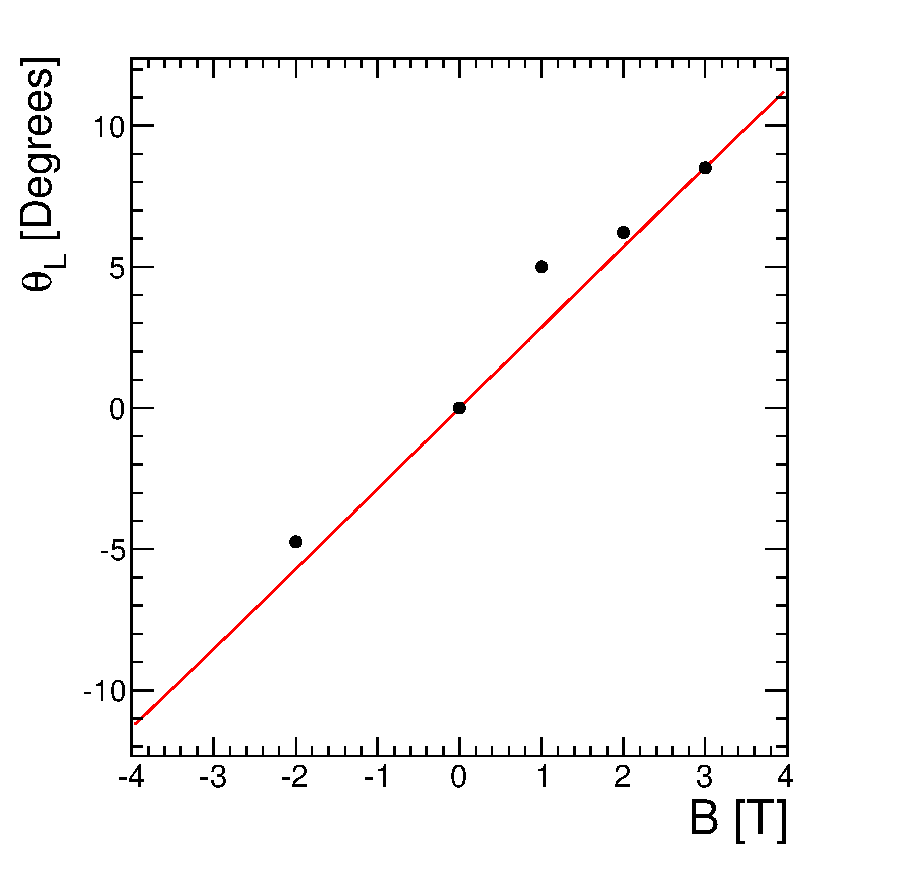
\includegraphics[width=0.5\textwidth]{plt-lorentz-angle-v4}
%\caption{ The Lorentz angle as a function of magnetic field.  The red line is a line representing the theoretical% value of $\theta_L = \tan^{-1} (\bar{\mu}\cdot B)$.  A value of $\bar{\mu} = 480$cm$^2$/Vs was assumed.  }
%\label{fig:lorentz_angles}
%\end{figure}

%
% Production Status
%
\section{Production Status}
As the 2011-2012 shutdown is too short to install the full PLT in its final location, a subset of the full PLT will first be installed approximately 15m away from the interaction point in order to gain operational experience in the LHC environment.  This installation requires two PLT cassettes with two telescopes apiece, such as the cassette pictured in Figure~\ref{fig:plt_cassette}.  A fully assembled PLT cassette consists of 12 detector planes, in addition to all of the supporting readout electronics, such as the FED, optical boards, etc.  The final PLT installation will require four full PLT cassettes for a total of 48 detector planes.  


As of October 2011, the PLT has a total of 53 qualified detector planes.  A plane is accepted if 
\begin{itemize}
\item After bump bonding, the ROC still functions
\item Full charge collection occurs at $<0.45$ V/$\mu$m
\item No dead double columns are found
\item Less than 1\% of the pixels are dead
\end{itemize}
By the end of 2011, there will be a total of 61 detector planes, ensuring 48 production planes and 13 planes to be used as spares or for further detector studies.  Production versions of all aspects of the frontend electronics--Hybrid Boards, HDIs, Port Cards, and Optical Motherboards--have also been produced.  Thus far, three fully read out production PLT cassettes have been constructed, and the fourth is ready to assembled. 

%
% Conclusions
%
\section{Conclusions}
We have studied both prototype and production versions of the PLT telescope, and in doing so established the functionality of the PLT and diamond detectors as a whole.  All measurements have shown that the PLT performs as necessary for establishing the desired $<1$\% systematic error on its luminosity measurement.   The measurement of the Lorentz angle smearing is a demonstration of the tracking capabilities of a diamond pixel detector. 
%Production of the PLT is progressing--one full cassette is ready to be installed on the CASTOR table, and over three quarters of the full detector is ready for installation in the inner layer of CMS.  
Two PLT cassettes are ready for installation in a temporary location in CMS in early 2012. The full set of four cassettes will be ready for installation in the final location in CMS during the 2013-2014 LHC shutdown.
Once installed inside of CMS, the PLT will be the first use of a diamond pixel detector in a high energy physics experiment.

\section*{Acknowledgment}
We thank the following people for their contributions 
to the PLT project: A.~Macpherson and N.~Rodrigues from CERN; S.~Schmid from HEPHY Vienna; E.~Halkiadakis and Y.~Gershtein from Rutgers~University.  
We thank the staff of the Princeton Institute for the Science and Technology of Materials (PRISM) for their assistance with the bump bonding.  
We thank the mechanical and electronic workshops at the University of Tennessee for their support.
 We are grateful to the University of Zurich group of Professor Amsler for lending us the strip detector telescope modules. Particularly,
the support by C.~Regenfus for the electronics readout and J.~Rochet for machining a support for the
telescope made this test beam possible. We are grateful to CMS Technical Coordination and US CMS for assistance in launching and sustaining the project.
We thank the CERN PS and SPS accelerator test beam group, D.~Lazic and colleagues, and the Fermilab Test Beam Facility test beam group for their excellent operation.

  
\begin{thebibliography}{1}

%\bibitem{plt-nim}
%R.Hall-Wilton \emph{et al.}, ``Results from a beam test of a prototype PLT diamond pixel telescope",   Nucl. Instrum. Meth. A (2010)  ,  doi:10.1016/j.nima.2010.04.097

\bibitem{DiamondDetectors}
W. de Boer \emph{et al.}, ``Radiation Hardness of Diamond and Silicon sensors compared." Phys. Stat. Sol. {\bf 204} (2007) 3004.

\bibitem{control-readout}
D.~Kotlinski \emph{et al.}, ``The control and readout systems of the CMS pixel barrel detector," Nucl.\ Instrum.\ Meth.\  A {\bf 565} (2006) 73.

\bibitem{psi46}
M.~Barbero \emph{et al.}, ``Design and test of the CMS pixel readout chip," Nucl. Instrum. Meth. A
{\bf 517} (2004) 349.

\bibitem{zurich-telescope}
C.~Amsler \emph{et al.}, ``A high resolution silicon beam telescope," Nucl.\ Instrum.\ Meth.\  A {\bf 480} (2002), 501-507.

\bibitem{diamond-mobility}
Pernegger, H. \emph{et al.}, ``Charge-carrier properties in synthetic single-crystal diamond measured with the transient-current technique," Journal of Applied Physics , vol.97, no.7, pp.073704-073704-9, Apr 2005
doi: 10.1063/1.1863417

\bibitem{pixel-2010}
W. Bugg \emph{et al.}, ``Studies of mono-crystalline CVD diamond pixel detectors", Nuclear Instruments and Methods in Physics Research Section A: Accelerators, Spectrometers, Detectors and Associated Equipment, Volume 650, Issue 1, 11 September 2011, Pages 50-54, ISSN 0168-9002, 10.1016/j.nima.2010.12.161.

\bibitem{ieee2010}
Hall-Wilton,~R. \emph{et al.}, "Resolution studies of single-crystal CVD diamond," Nuclear Science Symposium Conference Record (NSS/MIC), 2010 IEEE , vol., no., pp.813-818, Oct. 30 2010-Nov. 6 2010
doi: 10.1109/NSSMIC.2010.5873872




\end{thebibliography}


\end{document}